% poster.tex -- conference poster for "O Mirror, Where Art Thou?"
% Content follows ../rasti_template.tex; figures are read from ../figures/.
% Build:  pdflatex poster.tex
%
% Size: 42 x 36 inches (landscape). To change it, edit the \geometry line
% below; the two \setlength lines must follow it so tikzposter recomputes
% its usable area for the new paper size.

\documentclass[25pt, a0paper, landscape, margin=0mm, innermargin=18mm,
  blockverticalspace=8mm, colspace=14mm, subcolspace=12mm]{tikzposter}
\geometry{landscape=false, paperwidth=42in, paperheight=36in}
\makeatletter
\setlength{\TP@visibletextwidth}{\textwidth-2\TP@innermargin}
\setlength{\TP@visibletextheight}{\textheight-2\TP@innermargin}
\makeatother

\usepackage[T1]{fontenc}
\usepackage[default]{sourcesanspro}
\usepackage{amsmath}
\usepackage{amssymb}
\usepackage{bm}
\usepackage{booktabs}
\usepackage{graphicx}
\usepackage{enumitem}
\usepackage{multicol}
\usepackage{qrcode}
\graphicspath{{../figures/}}

%%%%%%%%%%%%%%%%%%%% COLOURS AND STYLES %%%%%%%%%%%%%%%%%%%%

\definecolor{navy}{HTML}{0C234B}
\definecolor{accent}{HTML}{AB0520}
\definecolor{paper}{HTML}{F4F4F1}
\definecolor{tint}{HTML}{E8ECF3}

\definecolorstyle{OMirror}{
  \colorlet{colorOne}{navy}
  \colorlet{colorTwo}{accent}
  \colorlet{colorThree}{tint}
}{
  \colorlet{backgroundcolor}{paper}
  \colorlet{framecolor}{navy}
  \colorlet{titlefgcolor}{white}
  \colorlet{titlebgcolor}{navy}
  \colorlet{blocktitlebgcolor}{navy}
  \colorlet{blocktitlefgcolor}{white}
  \colorlet{blockbodybgcolor}{white}
  \colorlet{blockbodyfgcolor}{black}
  \colorlet{innerblocktitlebgcolor}{accent}
  \colorlet{innerblocktitlefgcolor}{white}
  \colorlet{innerblockbodybgcolor}{tint}
  \colorlet{innerblockbodyfgcolor}{black}
  \colorlet{notefgcolor}{black}
  \colorlet{notebgcolor}{tint}
  \colorlet{notefrcolor}{accent}
}
\usecolorstyle{OMirror}

\definetitlestyle{OMirrorTitle}{
  width=\paperwidth, roundedcorners=0, linewidth=0pt, innersep=9mm,
  titletotopverticalspace=0mm, titletoblockverticalspace=14mm,
  titlegraphictotitledistance=10pt
}{
  \draw[draw=none, fill=titlebgcolor]
    (\titleposleft,\titleposbottom) rectangle (\titleposright,\titlepostop);
  \draw[accent, line width=10mm]
    (\titleposleft,\titleposbottom) -- (\titleposright,\titleposbottom);
}
\usetitlestyle{OMirrorTitle}

\defineblockstyle{OMirrorBlock}{
  titlewidthscale=1, bodywidthscale=1, titleleft,
  titleoffsetx=0pt, titleoffsety=0pt, bodyoffsetx=0pt, bodyoffsety=0pt,
  bodyverticalshift=0pt, roundedcorners=0, linewidth=1.5mm,
  titleinnersep=8mm, bodyinnersep=9mm
}{
  \ifBlockHasTitle
    \draw[draw=blocktitlebgcolor, line width=\blocklinewidth, fill=blockbodybgcolor]
      (blockbody.south west) rectangle (blocktitle.north east);
    \draw[draw=none, fill=blocktitlebgcolor]
      (blocktitle.south west) rectangle (blocktitle.north east);
    \draw[accent, line width=4mm]
      (blocktitle.south west) -- (blocktitle.south east);
  \else
    \draw[draw=blocktitlebgcolor, line width=\blocklinewidth, fill=blockbodybgcolor]
      (blockbody.south west) rectangle (blockbody.north east);
  \fi
}
\useblockstyle{OMirrorBlock}
\usebackgroundstyle{Default}

\setlist[itemize]{leftmargin=1.1em, itemsep=0.3em, topsep=0.3em,
  label={\color{accent}\raisebox{0.1ex}{\small$\blacktriangleright$}}}
\setlist[enumerate]{leftmargin=1.4em, itemsep=0.3em, topsep=0.3em}

% Small helpers
\newcommand{\um}{\,$\mu$m}
\newcommand{\cit}[1]{{\color{navy!70}[#1]}}
\newcommand{\figcap}[1]{\par\vspace{0.2em}{\small\color{black!75}#1\par}}
\newcommand{\keynum}[1]{{\color{accent}\bfseries #1}}
% Ragged-right block text avoids wide justification gaps in narrow columns
\newcommand{\rblock}[2]{\block{#1}{\raggedright #2}}

%%%%%%%%%%%%%%%%%%%% TITLE %%%%%%%%%%%%%%%%%%%%

\title{O Mirror, Where Art Thou?}
\author{Sai Krishanth P.M.\textsuperscript{1,2},
  Sanchit Sabhlok\textsuperscript{1},
  Jaren N. Ashcraft\textsuperscript{3},
  Kyle Van Gorkom\textsuperscript{1},
  Ewan S. Douglas\textsuperscript{1}}
\institute{\textsuperscript{1}Steward Observatory and
  \textsuperscript{2}Wyant College of Optical Sciences, University of Arizona \qquad
  \textsuperscript{3}UC Santa Barbara \qquad
  Contact: saikrishanth@arizona.edu}

% Replace tikzposter's default title layout (small caps, no subtitle).
\makeatletter
\renewcommand{\TP@maketitle}{%
  \centering
  \vbox{%
    \centering
    \color{titlefgcolor}
    {\bfseries\fontsize{80}{92}\selectfont \@title\par}
    \vspace*{0.2em}
    {\fontsize{42}{50}\selectfont Position retrieval using nested sampling and global minimization\par}
    \vspace*{0.6em}
    {\Large \@author\par}
    \vspace*{0.3em}
    {\large \color{white!80!navy}\@institute\par}
  }%
}
\makeatother

\tikzposterlatexaffectionproofoff
\begin{document}
\maketitle

% QR code to LinkedIn in the right end of the title bar. The white
% padding is the quiet zone that phone cameras need to read the code.
\node[anchor=north east, fill=white, inner sep=7mm]
  (qr) at ($(0.5\textwidth,0.5\textheight)+(-25mm,-7mm)$)
  {\qrcode[height=65mm]{https://www.linkedin.com/in/sai-krishanth-pulikesi-mannan-30609872/}};
\node[anchor=east, text=white, align=right, font=\large]
  at ($(qr.west)+(-8mm,0)$) {Connect on\\LinkedIn};

% Wyant College logo (white version for the navy title bar) at the left end
% of the title bar, vertically level with the QR code on the right.
% (The QR node spans 7 mm to 86 mm below the top edge, so its centre is
% 46.5 mm down.)
\node[anchor=west, inner sep=0pt]
  at ($(-0.5\textwidth,0.5\textheight)+(25mm,-46.5mm)$)
  {
\includegraphics[height=42mm]{wyant_logo_reverse.png}};

\begin{columns}

%%%%%%%%%%%%%%%%%%%% LEFT COLUMN %%%%%%%%%%%%%%%%%%%%
\column{0.3}

\rblock{Motivation}{
  {\large\bfseries\color{accent} Can we tell where a telescope's mirrors
  are from its images alone?\par}
  \vspace{0.4em}
  A misaligned mirror distorts the point spread function (PSF) differently
  across the field. Phase retrieval recovers the wavefront, not the mirror
  positions.
  \vspace{0.3em}

  \textbf{What we did:} infer rigid-body mirror positions \emph{directly}
  from multi-field PSFs.
  \begin{itemize}
    \item Ray-traced \textit{Hubble} (5 secondary-mirror DoF) and a compact TMA
      (10 primary + secondary DoF) in Optiland \cit{1}.
    \item Compared multi-field PSF coefficients via a Gaussian likelihood.
    \item Mapped the posterior with nested sampling, then refined it with
      differential evolution.
    \item Checked each solution by the residual wavefront error.
  \end{itemize}
}

\rblock{Validating on \textit{Hubble}}{
  Ritchey--Chr\'etien model (2.4\,m pupil, $\lambda = 0.55\,\mu$m) with
  five secondary-mirror degrees of freedom: decenter $(sdx, sdy)$, despace
  $sdz$ and tilts $(stx, sty)$. Noise-free PSFs at 5 fields, 15
  circular-Bessel modes, priors of $\pm200$\um\ and $\pm0.167^{\circ}$.
  \begin{itemize}
    \item Nautilus (42\,800 likelihood calls, $\ln\mathcal{Z}\approx+107.5$)
      tightly constrains both tilts and, more loosely, $sdz$.
    \item $sdx$ and $sdy$ stay nearly flat across the $\pm200$\um\ prior.
    \item DE starts from the median of the final 100 posterior samples,
      $(131.13,\,56.64,\,40.87,\,0.12,\,-0.03)$, which alone cuts the
      on-axis OPD RMS from 2.26 to 0.12 waves.
  \end{itemize}
  \begin{center}
    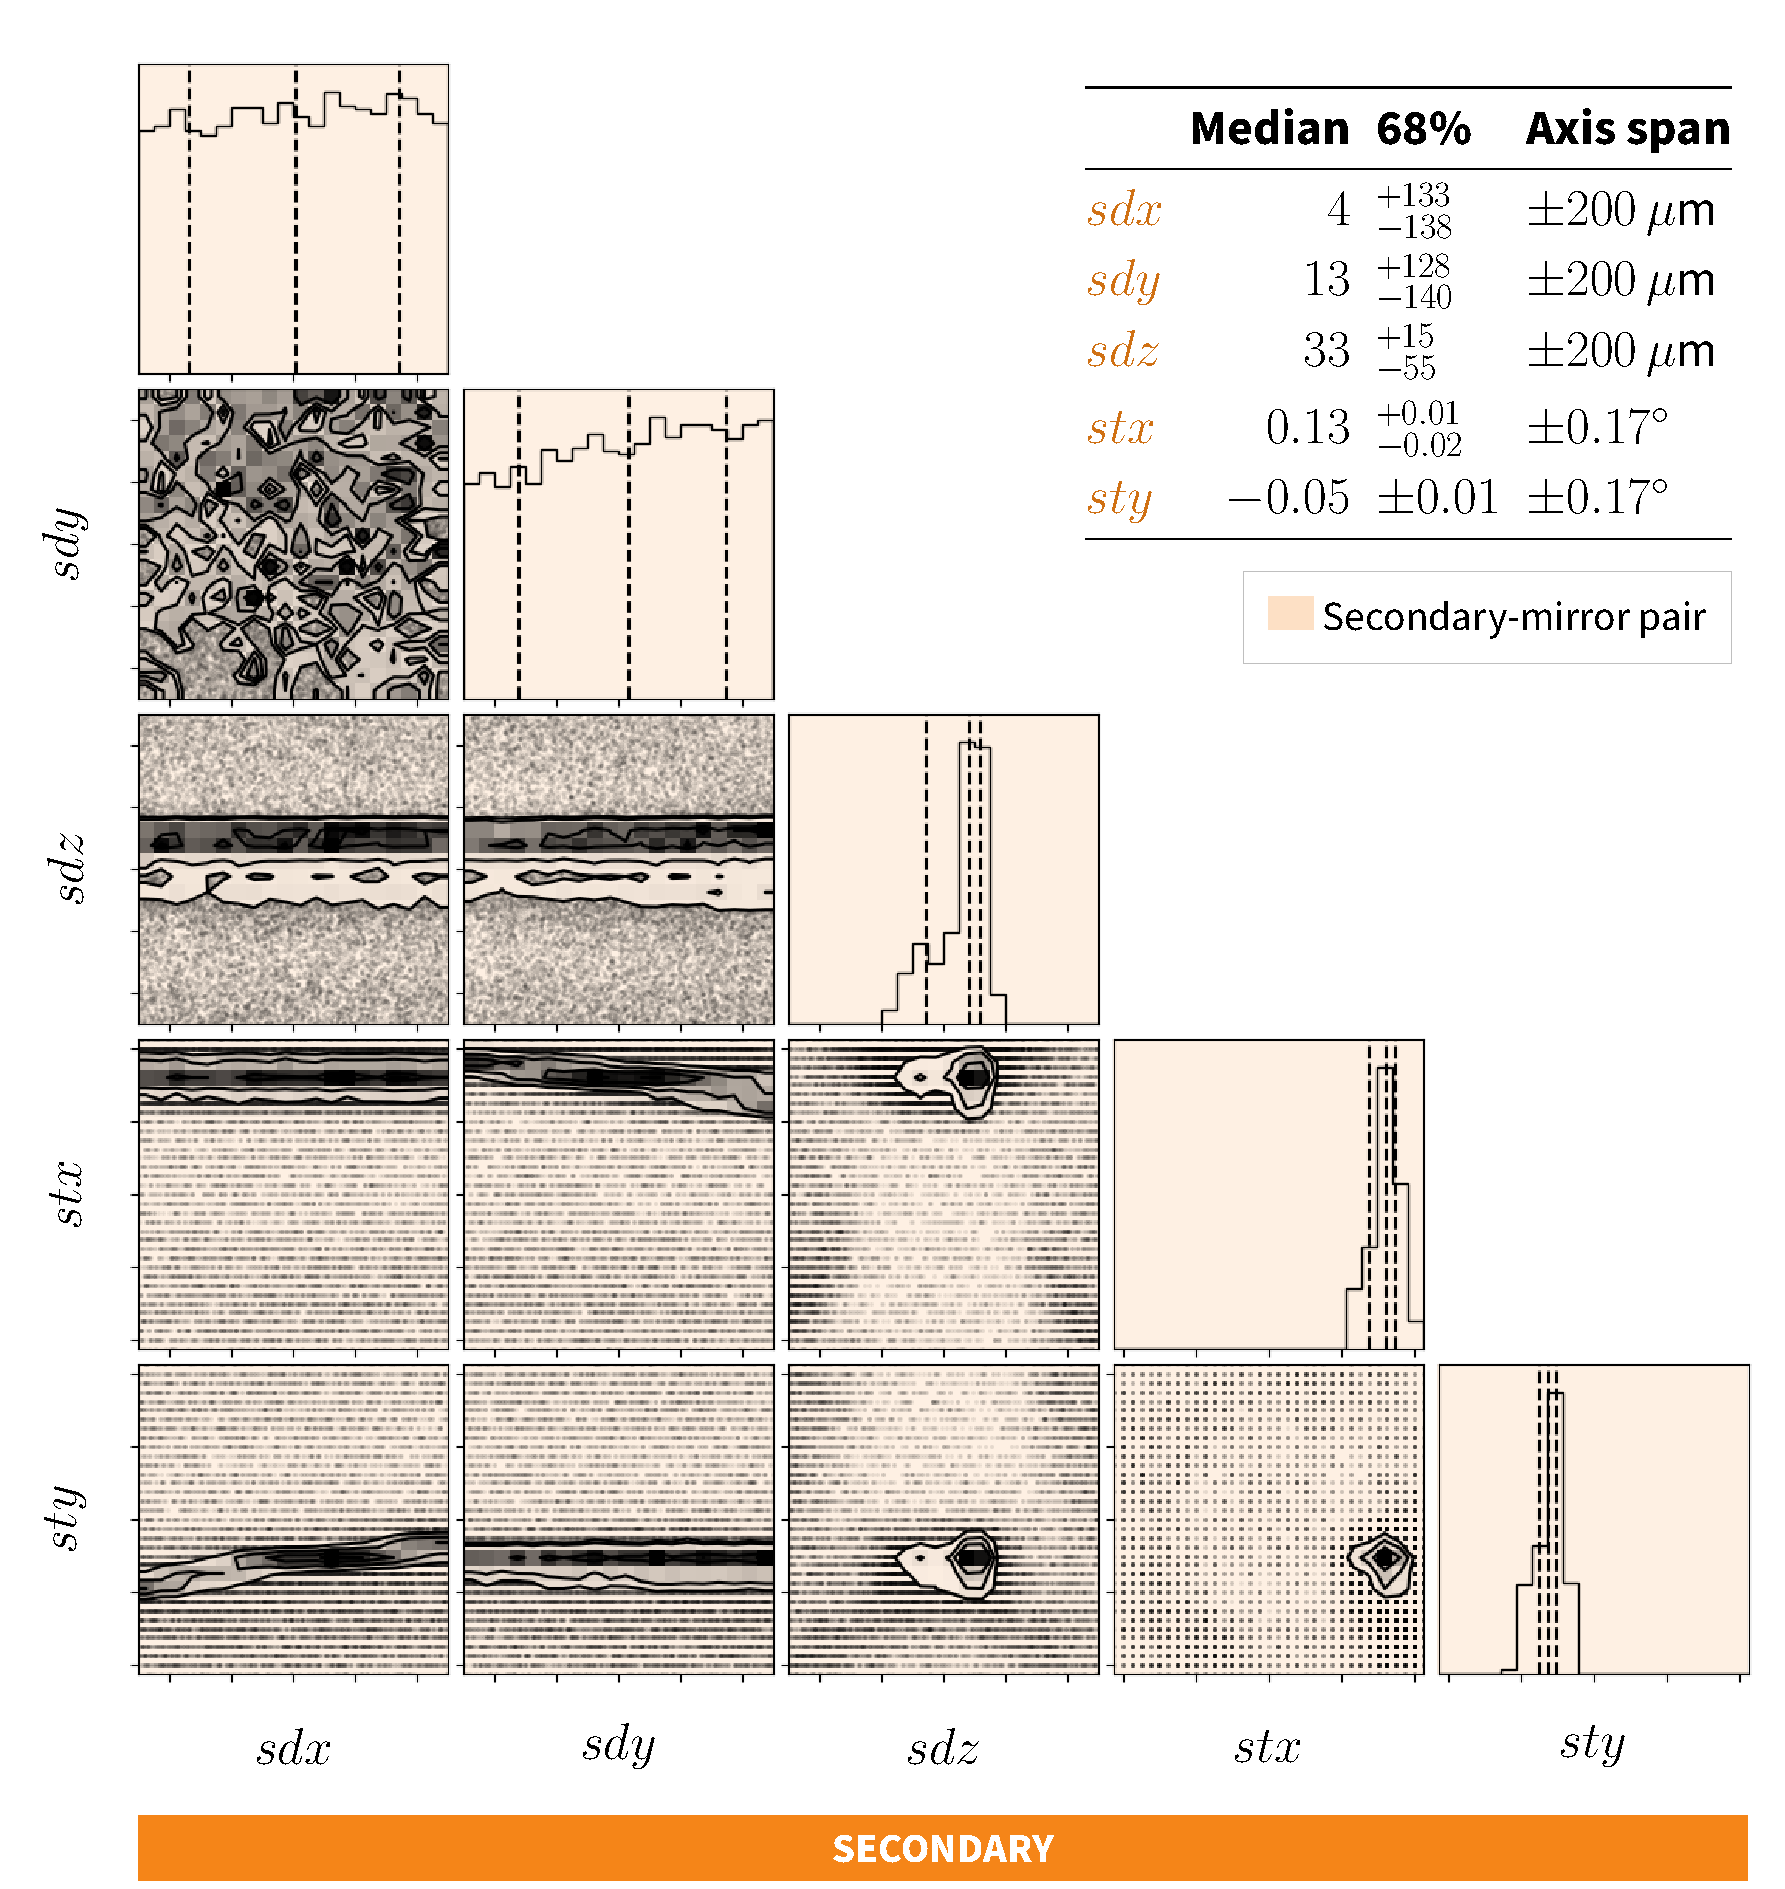
\includegraphics[width=0.96\linewidth]{hubbletilus_annotated.pdf}
  \end{center}
  \figcap{Nautilus posterior for the five secondary-mirror parameters; the
    table gives full-posterior medians and 68\% intervals.}
  \vspace{0.3em}
  Even so, DE using only the on-axis field recovers every translation to
  within $0.01\,\mu$m of the truth (centre panel).
}

%%%%%%%%%%%%%%%%%%%% CENTRE: METHOD, FEATURE FIGURE, REFERENCES %%%%%%%%%%%%%%%%%%%%
\column{0.4}

\rblock{Inference pipeline}{
  \begin{center}
    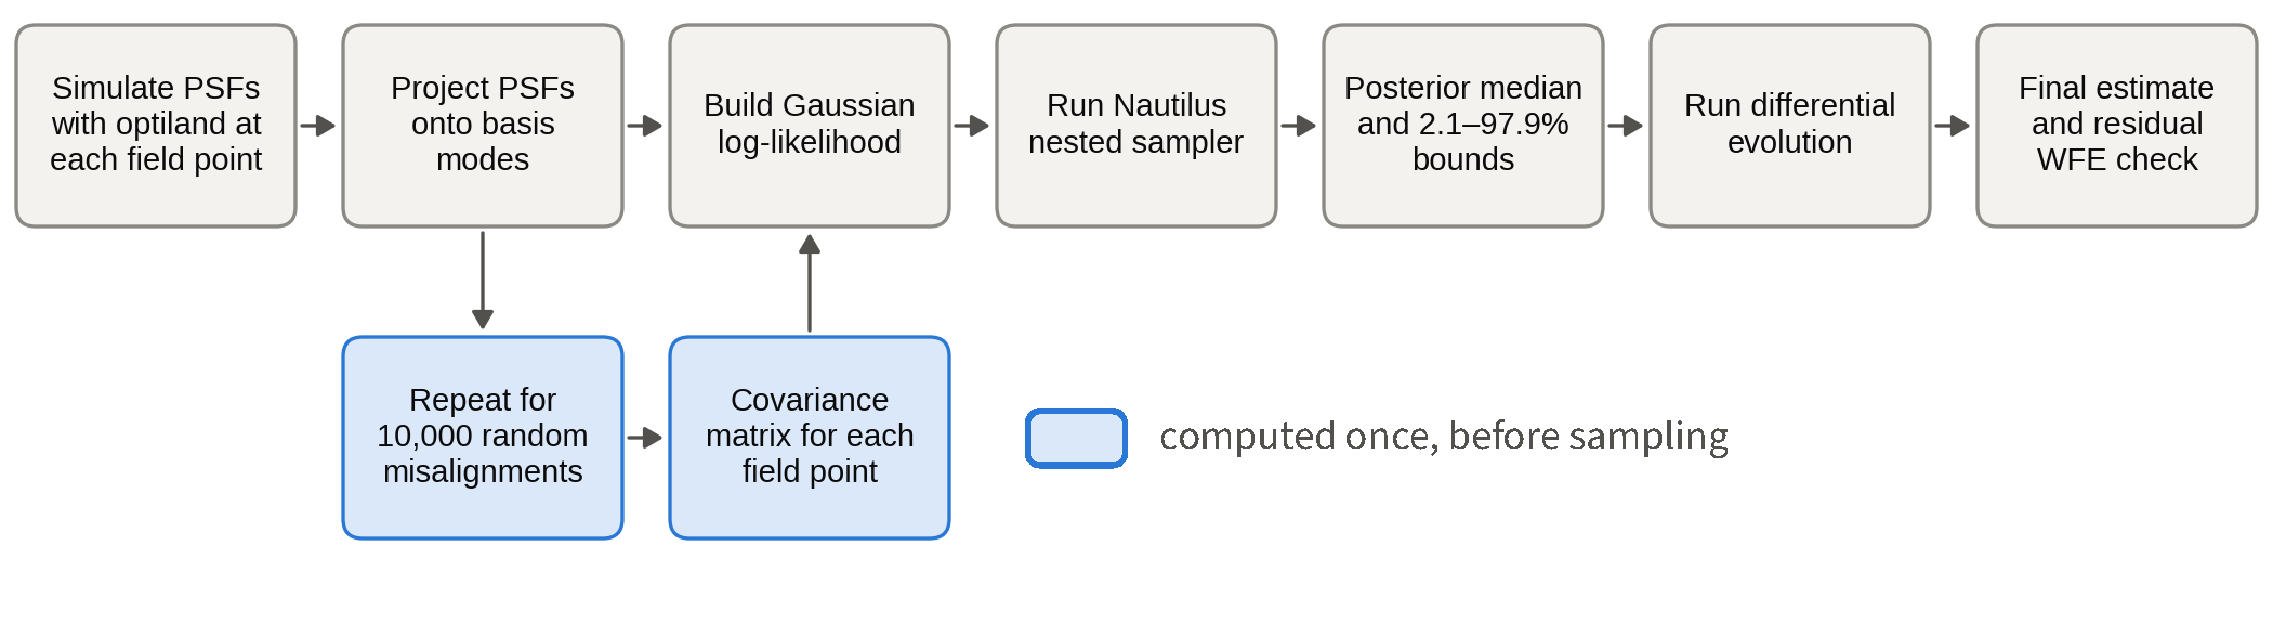
\includegraphics[width=\linewidth]{block_diagram_annotated.pdf}
  \end{center}
  \vspace{0.2em}
  \begin{minipage}[t]{0.49\linewidth}\raggedright
    Optiland \cit{1} PSF coefficients enter a Gaussian likelihood:
    \begin{gather*}
      \ln\mathcal{L}(\bm{\theta}) = \sum_{f\in\mathcal{F}}
      -\tfrac{1}{2}\,\Delta\mathbf{c}_f^{\top}\,\bm{\Sigma}_f^{-1}\,
      \Delta\mathbf{c}_f + \mathrm{const}, \\
      \Delta\mathbf{c}_f = \mathbf{c}_f(\bm{\theta}) - \mathbf{c}_{f,\mathrm{obs}}
    \end{gather*}
    $\bm{\Sigma}_f$ from $10^4$ random misalignments.
  \end{minipage}\hfill
  \begin{minipage}[t]{0.47\linewidth}\raggedright
    \begin{itemize}
      \item \textbf{Nested sampling} (Nautilus \cit{2,3}) maps the
        posterior.
      \item \textbf{Differential evolution} \cit{4,5} refines the
        Nautilus starting point.
      \item \textbf{Validation:} on-axis OPD RMS of the residual
        telescope.
    \end{itemize}
  \end{minipage}
}

% Feature block: accent-coloured frame and title bar.
\colorlet{blocktitlebgcolor}{accent}
\rblock{Algorithm recovers \textit{Hubble}'s optical alignment to numerical precision}{
  \begin{center}
    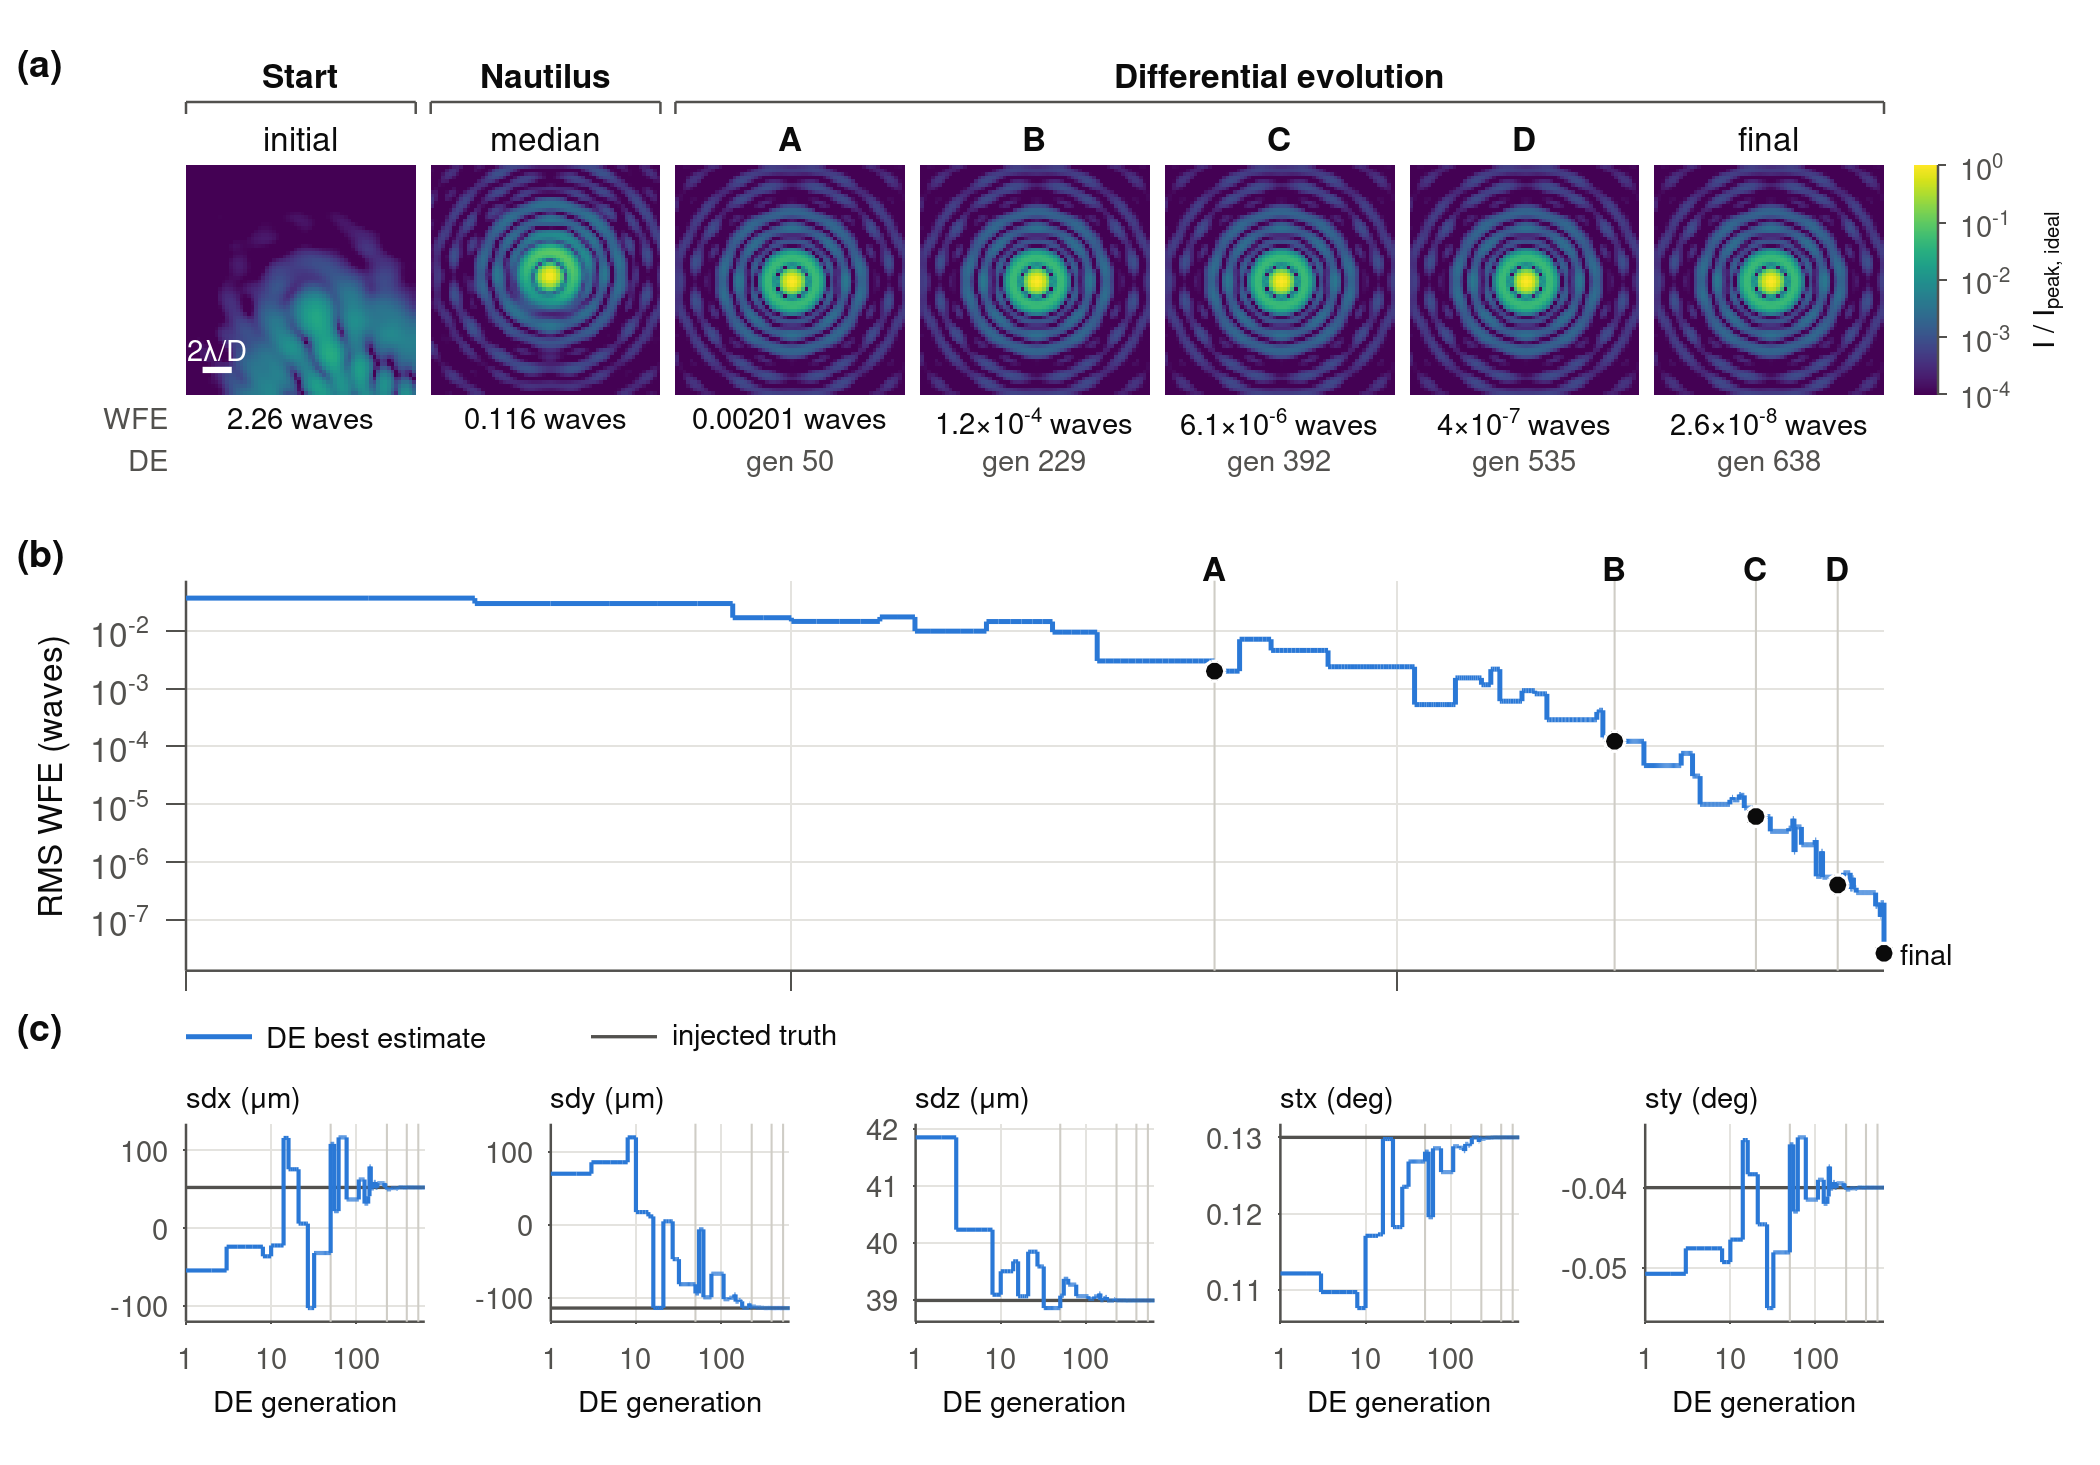
\includegraphics[width=\linewidth]{psf_progression.png}
  \end{center}
  \vspace{0.2em}
  \begin{minipage}[t]{0.55\linewidth}\raggedright
    \textbf{(a)} On-axis PSF, uncorrected (2.26 waves) to final DE
    solution ($2.6\times10^{-8}$ waves). \textbf{(b)} RMS wavefront error
    per DE generation. \textbf{(c)} Parameters converging to the injected
    truth.
  \end{minipage}\hfill
  \begin{minipage}[t]{0.42\linewidth}\raggedright
    Translations recovered to \keynum{$<0.01\,\mu$m}:
    \begin{center}
      \small
      \begin{tabular}{lrr}
        \toprule
         & \textbf{Truth} & \textbf{Recovered (DE)} \\
        \midrule
        $sdx$ ($\mu$m) & $52.22$ & $52.22$ \\
        $sdy$ ($\mu$m) & $-113.86$ & $-113.86$ \\
        $sdz$ ($\mu$m) & $38.99$ & $38.99$ \\
        $stx$ (deg) & $0.13$ & $0.13$ \\
        $sty$ (deg) & $-0.04$ & $-0.04$ \\
        \bottomrule
      \end{tabular}
    \end{center}
  \end{minipage}
}
\colorlet{blocktitlebgcolor}{navy}

\rblock{References}{
  \small
  \begin{multicols}{2}
  \begin{enumerate}[label={[\arabic*]}, leftmargin=1.9em, itemsep=0.5em, topsep=0em]
    \item Harrison 2026, Optiland v0.6.0
    \item Lange 2023, MNRAS 525, 3181
    \item Skilling 2006, Bayesian Analysis 1, 833
    \item Storn \& Price 1997, J. Global Optim. 11, 341
    \item Virtanen et al. 2020, Nature Methods 17, 261
    \item Kim, Choi \& Douglas 2023, Proc. SPIE 12677, 126770E
  \end{enumerate}
  \end{multicols}
  \vspace{0.2em}
  We thank T.~Eifler, N.~Franz, K.~Derby and S.~Blomquist.
}

%%%%%%%%%%%%%%%%%%%% RIGHT COLUMN %%%%%%%%%%%%%%%%%%%%
\column{0.3}

\rblock{Validating on a TMA}{
  Compact TMA \cit{6} (6.47\,m pupil, $\lambda = 0.65\,\mu$m) with ten
  degrees of freedom: decenter, despace and tilt of both the primary and the
  secondary. PSFs at 10 field points carry Gaussian noise
  ($\sigma = 0.01$ per pixel) and are projected onto 11 Zernike modes.
  \begin{itemize}
    \item Nautilus: 93\,200 likelihood calls, $\ln\mathcal{Z}\approx+484.7$.
    \item DE recovers all translations to \keynum{$\lesssim 17\,\mu$m} and
      reduces on-axis OPD RMS from 8.24 to $7\times10^{-3}$ waves.
  \end{itemize}
  \begin{center}
    \small
    \begin{tabular}{lrrrr}
      \toprule
      & \multicolumn{2}{c}{\textbf{Primary}} & \multicolumn{2}{c}{\textbf{Secondary}} \\
      \cmidrule(lr){2-3}\cmidrule(lr){4-5}
      & Truth & Recovered & Truth & Recovered \\
      \midrule
      $dx$ ($\mu$m) & $-152.75$ & $-159.43$ & $-42.31$ & $-38.01$ \\
      $dy$ ($\mu$m) & $316.91$ & $309.97$ & $923.33$ & $939.85$ \\
      $dz$ ($\mu$m) & $26.63$ & $24.77$ & $-32.75$ & $-34.56$ \\
      $tx$ (deg) & $2.98{\times}10^{-5}$ & $2.22{\times}10^{-4}$ & $0.0269$ & $0.0272$ \\
      $ty$ (deg) & $1.61{\times}10^{-5}$ & $6.80{\times}10^{-5}$ & $0.0098$ & $0.0098$ \\
      \bottomrule
    \end{tabular}
  \end{center}
  \begin{center}
    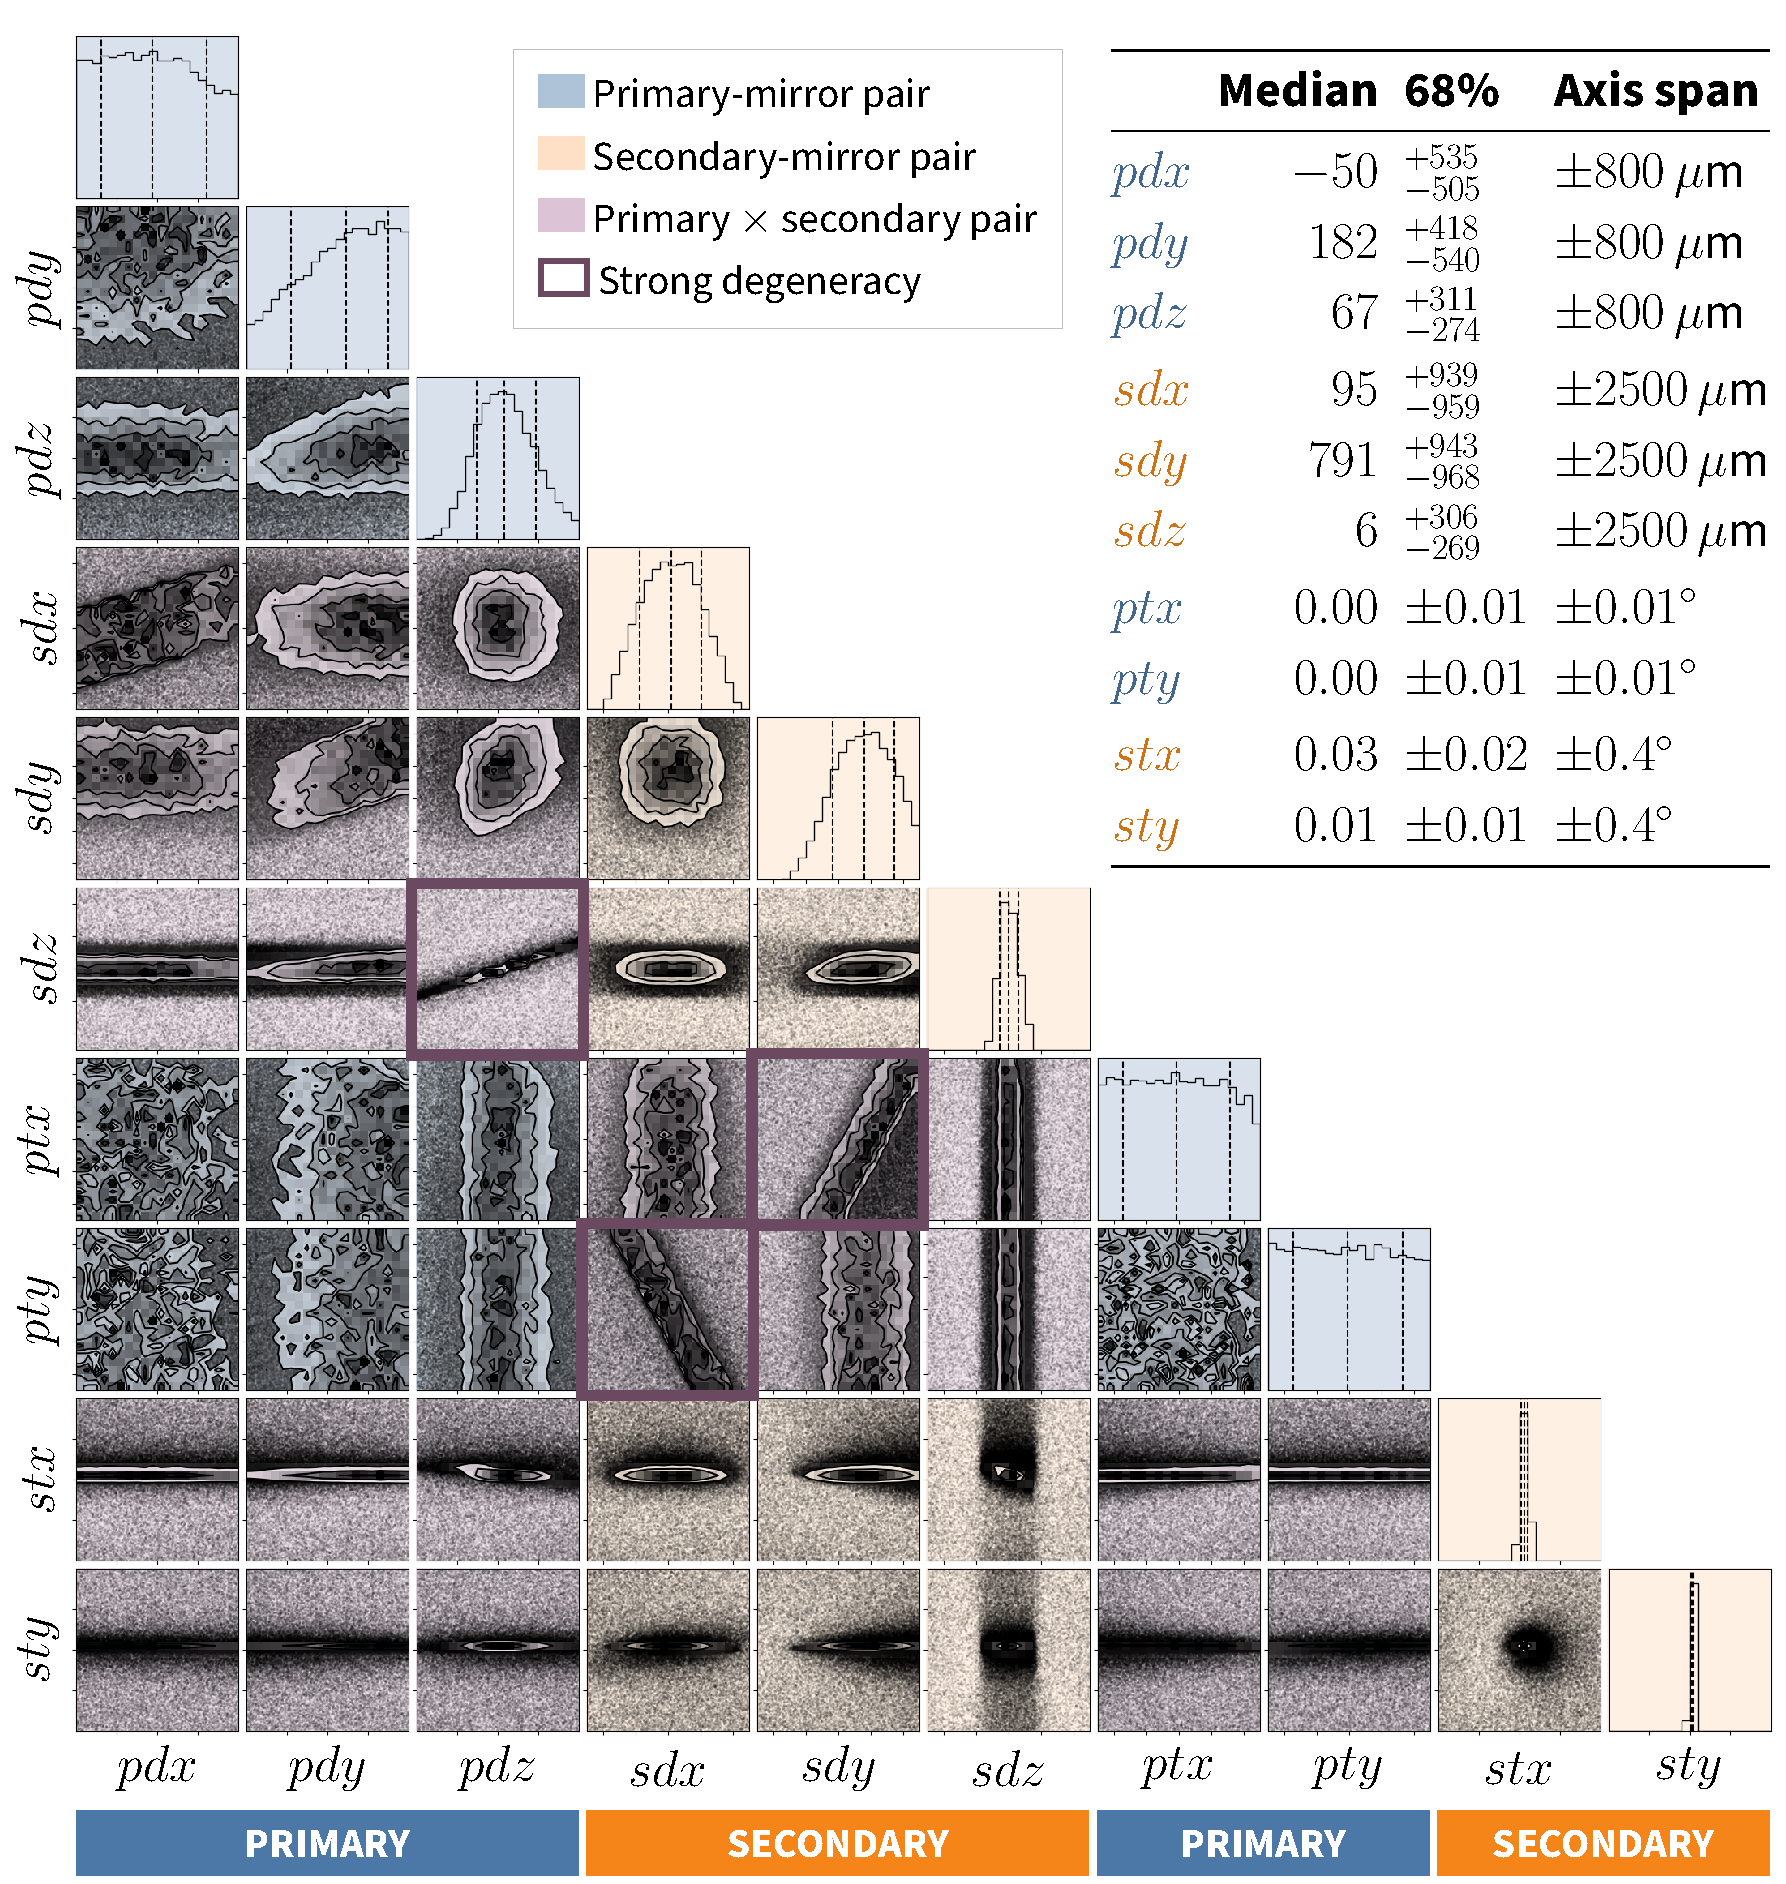
\includegraphics[width=0.96\linewidth]{pearltilus_annotated.pdf}
  \end{center}
  \figcap{Nautilus posterior for the ten TMA parameters, shaded by mirror.
    Outlined panels are the strongest primary--secondary degeneracies.}
  \begin{itemize}
    \item $pdx$ and both primary tilts are nearly flat across their priors;
      only the secondary tilts are tightly constrained.
    \item Degeneracies: $pdz$--$sdz$ trade off in focus; $ptx$--$sdy$ and
      $pty$--$sdx$ trade off in coma, because a tilt of one mirror and a
      decenter of the other both add nearly field-constant coma.
  \end{itemize}
}

\rblock{Conclusions and next steps}{
  \begin{itemize}
    \item Mirror alignment is recovered directly from multi-field PSF
      coefficients.
    \item \textbf{\textit{Hubble}:} OPD RMS 2.26 $\to$ \keynum{$3\times10^{-8}$}
      waves.
    \item \textbf{TMA:} OPD RMS 8.24 $\to$ \keynum{$7\times10^{-3}$} waves.
    \item Degeneracies motivate multi-field sensing.
    \item Next: chromatic and realistic noise models, and laboratory and
      on-sky PSF data for future large space telescopes.
  \end{itemize}
}

\end{columns}

\end{document}
